
\chapter{Electricity system}
% Use \titlerunning{Short Title} for an abbreviated version of your contribution title if the original one is too long
%\author{Juan Van Roy, Bart Verbruggen and Johan Driesen}
%\authorrunning{J. Van Roy, B. Verbruggen, J. Driesen}
%\institute{Bart Verbruggen \at K.U.Leuven, Kasteelpark Arenberg 10 bus 2445, BE-3001 Leuven (Heverlee) \email{bart.verbruggen@esat.kuleuven.be}
%\and Juan Van Roy \at K.U.Leuven, Kasteelpark Arenberg 10 bus 2445, BE-3001 Leuven (Heverlee) \email{juan.vanroy@esat.kuleuven.be}}
%\maketitle

%\abstract{A numeric electric system model is developed in Modelica for integrated energy simulation.}

%\vspace{\baselineskip}

In this section, we describe in detail the electrical models that are implemented in Modelica as part of the IDEAS platform. These are models on the production, electrical distribution and storage side. First the photovoltaic (PV) system is treated which produces electricity locally from solar energy. In a second part, the distribution of electricity on distribution level is described.

Work in progress are the in-home electricity grid and the electrical storage in batteries.

\section{Photovoltaic system}
First, a photovoltaic (PV) system is implemented based on the five parameter model to simulate the energy production from a photovoltaic system under operational conditions. The five parameter model, which is temperature dependent, is based on the single diode equivalent circuit of a PV panel~\cite{desoto,sera}. The five parameters are:
\begin{itemize}
\item the light current, $I_{ph}$;
\item the diode reverse saturation current, $I_{o}$;
\item a shunt resistance, $R_{sh}$;
\item a series resistance, $R_{s}$;
\item the thermal voltage, $V_{t}$.
\end{itemize} 
These parameters are indicated in the equivalent circuit presented in Figure~\ref{fig:5param_equiv}.

\begin{figure}[ht]
\centerline{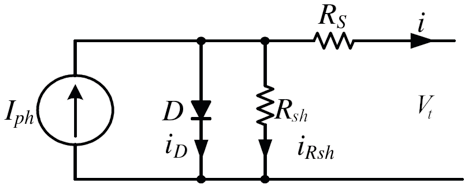
\includegraphics[width=0.65\textwidth]{Electric/MyGraphics/5param_eq.png}}
\label{fig:5param_equiv}
\caption{Five parameter model of a PV panel~\cite{desoto}} 
\end{figure}

\subsection{Power output of PV panel}
The electrical output from a PV system depends on the solar radiation, the ambient temperature of the cells, the solar incidence angle and the load. The solar radiation, incidence angle and temperature is obtained from chapter \ref{chap:climate}. The parameters needed for the model can generally be obtained from data gathered from the manufacturer's specifications of the solar panels. The required specifications to calculate the five parameters are the current $I_{mpp}$ and voltage $V_{mpp}$ at maximum power point (mpp) under standard testing conditions (STC)\footnote{Standard testing conditions are $(i)$ an irradiance of 1000 W/m$^2$ and $(ii)$ a cell temperature of 25$^\circ$C and $(iii)$ reference air mass of 1.5}, the short circuit current $I_{sc}$ and open circuit voltage $V_{oc}$ under the same standard testing conditions, the temperature coefficients $k_{i}$ and $k_{v}$ of respectively the short circuit current and open circuit voltage and the nominal cell temperature under STC $T_{c,ref}$.

The general current-voltage ($i-v$) equation for the single diode equivalent circuit is given in Eq.~(\ref{eq1}). This equation can be written for three points: $(i)$ short-circuit, $(ii)$ open-circuit and $(iii)$ maximum power point~\cite{sera}.

\begin{equation}
i(t) = I_{ph} - I_{0} \left(e^{\frac{v(t) + i(t)R_{s}}{n_{s} V_{t}}} - 1 \right) - \frac{v(t) + i(t)R_{s}}{R_{sh}}
\label{eq1}
\end{equation}
In this equation $V_{t}$ is the junction thermal voltage and $n_{s}$ the number of cells in the panel connected in series:
\begin{equation}
V_t = \frac{f_{A} k T_{stc}}{q}
\label{eqVt}
\end{equation}
with $f_A$ the ideality factor, $k$ the Boltzmann's constant ($1.380663 \cdot 10^{-23}$ J/K), $q$ the charge of an electron ($1.600218 \cdot 10^{-19}$ C) and $T_{stc}$ the cell temperature under STC.

The voltage $V_{mpp}$ and current $I_{mpp}$ at maximum power point should satisfy Eq.~(\ref{eq1}). The derivative of the power with respect to the voltage ($dP/dV$) at $V_{mpp}$ and $I_{mpp}$ should be zero Eq.~(\ref{pmpp}). The derivative of the current with respect to the voltage ($dI/dV$) at short circuit current should be the negative of the shunt conductance ($R_{sh}^{-1}$). These equations lead to the calculation of the parameters $R_{s}$, $R_{sh}$ and $V_{t}$.

The maximum power point $P_{mpp}$ (at $I = I_{mpp}$) can be found with Eq.~(\ref{pmpp}):
\begin{equation}
\frac{dP}{dV} = I_{mpp} + V_{mpp} \frac{-\frac{(I_{sc} R_{sh} - V_{oc} + I_{sc} R_{s}) e^{\frac{V_{mpp} + I_{mpp} R_{s} - V_{oc}}{n_{s} V_{t}}}}{n_{s} V_{t} R_{sh}} - \frac{1}{R_{sh}}}{1 + \frac{(I_{sc} R_{sh} - V_{oc} + I_{sc} R_{s}) e^{\frac{V_{mpp} + I_{mpp} R_{s} - V_{oc}}{n_{s} V_{t}}}}{n_{s} V_{t} R_{sh}} + \frac{R_{s}}{R_{sh}}}
\label{pmpp}
\end{equation}

The reverse saturation current $I_{o}$ and light current $I_{ph}$ at STC can be found based on Eq.~(\ref{eq1}) for the short circuit (Eq.~(\ref{eq4})) and open circuit condition (Eq.~(\ref{eq5})).
\begin{equation}
I_{sc} = I_{ph} - I_{0} e^{\frac{I_{sc} R_{s}}{n_{s} V_{t}}} - \frac{I_{sc} R_{s}}{R_{sh}}
\label{eq4}
\end{equation}
\begin{equation}
I_{oc} = 0 = I_{ph} - I_{0} e^{\frac{V_{oc}}{n_{s} V_{t}}} - \frac{V_{oc}}{R_{sh}}
\label{eq5}
\end{equation}

The PV parameters are adjusted to take into account the position of the sun, the direct and indirect radiation and the ambient temperature. The cell temperature has been adjusted to be the ambient temperature plus the losses of the panel. The parameters for the non-reference conditions are calculated in the next paragraphs.

The tilt angle and orientation of the PV panels are parameters of the PV model. Together with the sun's position, the incidence angle of the direct beam radiation can be calculated which allows to obtain the amount of radiation that gets reflected by and passes through the PV panel cover. This is done using incidence angle modifiers that are derived from De Soto et al.~\cite{desoto}. The incidence angle modifier $K_{\tau \alpha}(\theta)$ can be found from the transmittance $\tau$ of the cover system with Eq.~(\ref{eq8}), which is approximated in Eq.~(\ref{eq7}). The angle of refraction, $\theta _{r}$, is determined in Eq.~(\ref{eq6}) by Snell's law, with $\theta$ the incidence angle and $n$ the effective index of refraction of the cell cover. In Eq.~(\ref{eq7}), $f_K$ is the glazing extinction coefficient and $f_L$ is the glazing thickness. In the model $f_K$ and $f_L$ can be adjusted. By default, $f_K$ is assumed to be $4~m^{-1}$ and $f_L$ is assumed to be $2~mm$.
\begin{equation}
\theta _{r} = \arcsin(n \sin \theta)
\label{eq6}
\end{equation}
\begin{equation}
\tau (\theta) = e^{-\frac{f_K f_L}{\cos \theta _{r}}} \left[1 - \frac{1}{2} \left(\frac{\sin^{2}(\theta _{r} - \theta)}{\sin^{2}(\theta _{r} + \theta)} + \frac{\tan^{2}(\theta _{r} - \theta)}{\tan^{2}(\theta _{r} + \theta)} \right) \right]
\label{eq7}
\end{equation}
\begin{equation}
K_{\tau \alpha}(\theta) = \frac{\tau (\theta)}{\tau (0)}
\label{eq8}
\end{equation}

The incidence angle modifiers and the direct and diffuse radiation, which are inputs to the model, allow together with the reflected radiation to calculate the absorbed solar radiation $S$ in Eq.~(\ref{eq9}). In this equation $G_{b}$ is the direct, $G_{d}$ the diffuse and $G$ the total radiation. The slope of the PV panel is characterized by $\beta$.
\begin{equation}
\frac{S}{S_{ref}} = \frac{G_{b}}{G_{ref}} K_{\tau \alpha , b} + \frac{G_{d}}{G_{ref}} K_{\tau \alpha , d} \frac{1 + \cos \beta}{2} + \frac{G}{G_{ref}} \rho K_{\tau \alpha , g} \frac{1 - \cos \beta}{2}
\label{eq9}
\end{equation}
with
\begin{equation}
S_{ref} = G_{ref} e^{-f_K f_L}
\label{eqSref}
\end{equation}
and $G_{ref}$ is the irradiance at STC (1000 W/m$^2$).

The light current $I_{ph}$, reverse saturation current $I_{0}$ and thermal voltage $V_{t}$ at non-reference conditions can be calculated when the temperature, open circuit voltage and short circuit current are known~\cite{sera}. The open circuit voltage $V_{oc}$ can be calculated using Eqns.~(\ref{eq10}) and~(\ref{eq11}). The short circuit current $I_{sc}$ can be found using Eq.~(\ref{eq12}).
\begin{equation}
e^{\frac{V_{oc}(S)}{n_{s} V_{t}}} = \frac{I_{ph}(S) R_{sh} - V_{oc}(S)}{I_{0} {R_{sh}}}
\label{eq10}
\end{equation}
\begin{equation}
V_{oc}(T) = V_{oc} + k_{v} (T - T_{stc})
\label{eq11}
\end{equation}
\begin{equation}
I_{sc}(S,T) = I_{sc} \left(\frac{S}{S_{ref}} \right) \left(1 + \frac{k_{i}}{100} (T - T_{ref}) \right)
\label{eq12}
\end{equation}

The reverse saturation current $I_{0}$ can be calculated with Eq.~(\ref{eq13}). The light current $I_{ph}$ is found using Eq.~(\ref{eq14}).
\begin{equation}
I_{0} = \left(I_{sc} - \frac{V_{oc} - I_{sc} R_{s}}{R_{sh}} \right) e^{-\frac{V_{oc}}{n_{s} V_{t}}}    
\label{eq13}
\end{equation}
\begin{equation}
I_{ph} = I_{0} e^{\frac{V_{oc}}{n_{s} V_{t}}} + \frac{V_{oc}}{R_{sh}}
\label{eq14}
\end{equation}

\subsection{Power output of PV system}
A PV system consists of multiple PV panels connected in series. Assuming that all PV panels are in the same condition, the output DC voltage can be multiplied by the number of PV panels in a PV system.

The number of PV panels is a parameter of the general PV system model. The peak power $P_{peak}$ is defined with $V_{mpp}$, $I_{mpp}$ and the number of panels $n_p$:
\begin{equation}
P_{peak} = n_p V_{mpp} I_{mpp}
\label{Ppeak}
\end{equation}

\subsection{Orientation PV system}
The PV system has two orientation parameters, namely $(i)$ the azimuth and $(ii)$ the inclination angle. An azimuth angle of 0$^\circ$ is defined as towards the South, -90$^\circ$ for the East and 90$^\circ$ for the West. Applied to Belgium, the PV system has the highest annual electricity production when the system is oriented directly to the South with an inclination of 34$^\circ$.

The inclination and azimuth angles are paremeters of the modeled photovoltaic system.

\subsection{Inverter}
A PV system is connected to the electrical grid through an inverter, which converts the generated DC power to AC power with an efficiency $\eta_{dc/ac}$.

Due to the lack of simultaneity of production and consumption, a bidirectional energy flow may occur between a building and the electrical grid (e.g. low voltage grid for residential buildings), which may lead to voltage instabilities on the grid (e.g. increasing voltages due to the injection of electricity, unbalance, etc.). To avoid excessive feeder voltages at the moments of re-injecting PV power in the grid, the inverter is curtailed when a predefined voltage limit is reached. Curtailing of a PV system means production losses.

%According to the AREI\footnote{Algemeen Reglement voor Elektrische Installaties, Belgi\"e.}, Art.235, this limit is 6 \% above the nominal voltage (230 V in Belgium). A certain minimal off-time is given before reconnecting the inverter to the grid. Synergrid states that PV systems are curtailed when the average grid voltage at the connection point of the building (during 10 minutes) reaches a predefined voltage of 230 + 10 \% V)~\cite{synergrid}. An instant switch-off is required when the voltage reaches 230 + 15 \% V. In principle, the strictest rule has to be followed. In this case, there is an agreement that the values of Synergrid can be followed until the AREI is adapted.

\section{Electrical distribution grid}
In the electrical grid system two types of grids exist, namely $(i)$ distribution and $(ii)$ transmission grids~\cite{ehaesen,willis}. However, in Belgium, distribution grids differ fundamentally from transmission grids:

\begin{itemize}
\item They are mostly radially: This means there is only one feeding transformer\footnote{Traditionally, there is only a unidirectional power flow.}. Due to the lack of a redundant supply, the reduced reliability is a major disadvantage. In case of a fault, all loads behind the fault will be switched off.
\item The lower the voltage level, the higher the R/X ratio. Thus, low voltage residential distribution grids are highly resistive.
\end{itemize}

An electrical distribution grid for low voltage is modeled. E.g. a residential district is typically a radial distribution grid with a rated nominal voltage of 230/400 V\footnote{230 V phase voltage, 400 V line voltage.} wye (or star) connection. Both a single-phase en three-phase grid can be simulated. The single-phase grid can serve for fully balanced simulations.

First, the grid topology is described. As will be shown, any radial grid can be easily represented by two matrices, namely the incidence and impedance matrix. Second, the background for the power flow analysis will be described to determine the nodal currents, line currents and nodal voltages. Radial grids are, compared to meshed grids, more easy to analyze and because of the low cost, it is prefered for distribution grids~\cite{ehaesen}. Figure~\ref{figIEEE} gives an example of a radial grid. This figure shows an IEEE 34 node test feeder~\cite{IEEE_testfeeder}.

\begin{figure}[ht]
\centerline{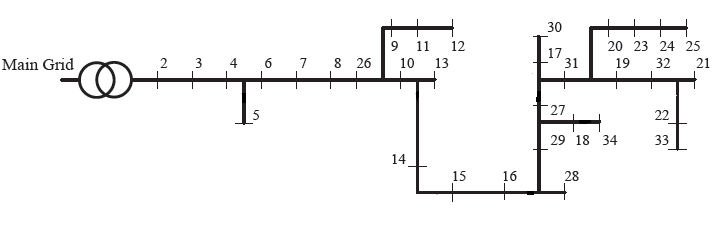
\includegraphics[width=0.75\textwidth, angle=0]{Electric/MyGraphics/grid_ieee34.png}}
\caption{Grid topology IEEE 34 node test feeder~\cite{IEEE_testfeeder}}
\label{figIEEE}
\end{figure}

\subsection{Grid topology}
Distribution grids for low-voltage are mostly radial grids. In this case, a residential three-phase distribution grid is modeled. A residential district is typically a radial feeder with a rated no\-mi\-nal voltage of 230/400V wye (or star) connection. For distribution grids without distributed generation (uni-directional power flow), the voltage at the feeder typically has a higher value to ensure that the voltage in the whole feeder stays within the preset boundaries. For a fully balanced system, the single-phase equivalent grid can be used. Connections to loads (e.g. buildings) are represented by nodes. Loads and generation units can be single or three-phase connected to the grid.

Any radial grid can be represented by an incidence matrix (or connection matrix) \textbf{T}. The columns correspond with the number of nodes. Each line in \textbf{T} represents a segment of the grid (branch) between two nodes. Each segment is represented by 1 and -1 at respectively the start and end node of that segment. The other row elements are zero. A node can be the start or end node of more than one segment. Since there are $n$ nodes, a radial grid consists of $n-1$ line segments. To attain a square matrix, an additional (first) row is introduced to represent the imaginary line segment between the transformer and the first node. This line segment only has an end node.

Eq.~(\ref{eqT}) gives an example of the representation of an incidence matrix \textbf{T} in which the nodes are all next to each other, which means branches are between
consecutive nodes.

\begin{equation}
\textbf{T} = \begin{bmatrix}
-1 & 0 & 0 & \cdots & 0 & 0 & 0\\
1 & -1 & 0 & \cdots & 0 & 0 & 0\\
0 & 1 & -1 & \cdots & 0 & 0 & 0\\
\vdots & \vdots & \vdots & \ddots & \vdots & \vdots & \vdots\\
0 & 0 & 0 & \cdots & -1 & 0 & 0\\
0 & 0 & 0 & \cdots & 1 & -1 & 0\\
0 & 0 & 0 & \cdots & 0 & 1 & -1
\end{bmatrix}
\label{eqT}
\end{equation}

Cables, with a length $f_L$ ($m$), for the line segments of an electrical grid are characterized by an impedance $Z = R + jX$, with $R$ the resistance and $X$ the reactance of the cable:
\begin{equation}
R = f_L r
\label{eqR}
\end{equation}
\begin{equation}
X = f_L x
\label{eqX}
\end{equation}
with $r$ the characteristic resistance $x$ the characteristic reactance in $\Omega /m$. This allows to represent the grid with an impedance matrix $\textbf{Z} = \textbf{R} + j \textbf{X}$.

In a similar way, the houseconnectors are described. These are the connection lines between the in-home grid and the grid connection node of the building. The houseconnectors are characterized by a cable type, cable length and the type of connection with the grid (\mbox{single-phase} or three-phase connection).

\subsection{Power flow analysis}
A power flow analysis is required to characterize the impact of a load profile on each connection node in the grid. A power flow analysis is performed to determine the nodal currents $\textbf{I}_{node}$, line currents $\textbf{I}_{line}$ and nodal voltages $\textbf{V}_{node}$. The calculations are based on the Laws of Kirchhoff:
\begin{description}
\item[\textbf{Conservation of electric charge}] At any node, the sum of currents flowing into the node is equal to the sum of currents flowing out of the node (Eq.~(\ref{kirch1})).
\item[\textbf{Conservation of energy}] The sum of the voltage drops around any closed circuit is zero (Eq.~(\ref{kirch2})).
\end{description}

\begin{equation}
\sum_{k = 1}^{nodes} i_{k}(t) = 0
\label{kirch1}
\end{equation}
\begin{equation}
\sum_{k = 1}^{branches} \Delta v_{k}(t) = 0
\label{kirch2}
\end{equation}

The voltage drop in a branch $k$ between nodes $n$ and $n+1$ is defined as:
\begin{equation}
\Delta v_k(t) = Z_k i_{line,k}(t) = v_n(t) - v_{n+1}(t).
\end{equation}

When the nodal currents $\textbf{I}_{node}$, line currents $\textbf{I}_{line}$ and nodal voltages $\textbf{V}_{node}$ are known, the total flow of apparent power $S$ can be calculated. $S$ consists of active power $P$ and reactive power $Q$:
\begin{equation}
S(t) = \sum_{f = 1}^{phases}P_f(t) + j Q_f(t)% = \sum_{f = 1}^{phases}U_{phase} I^*
\end{equation}
The apparent power S is calculated as:
\begin{equation}
S = U_{phase} I^*
\end{equation}
with $U_{phase}$ the phase voltage and $I^*$ the complex conjugate of $I$.

The ohmic losses in a single-phase grid are calculated as follows:
\begin{equation}
P_{grid~loss,~1-phase} = \sum_{k = 1}^{branches} P_{k,~loss} = \sum_{k = 1}^{branches} R_k I_{k,~line}^{2} 
\label{Ploss}
\end{equation}
A three-phase distribution grid consists of three phases and a neutral cable. Therefore, Eq.~(\ref{Ploss}) can be rewritten for three-phase distribution grids as follows:
\begin{equation}
P_{grid~loss,~3-phase} = \sum_{f = 1}^{phases} P_{grid~loss,~f} + P_{neutral,~loss} 
\label{3Ploss}
\end{equation}

\subsection{Single/three-phase grid simulation}
Electrical loads, generation units, storage units (e.g. batteries) can be single-phase or three-phase connected to the grid. Generally the system is not fully balanced (e.g. the same load in each phase for each node in the distribution grid) and an unbalanced three-phase power flow analysis is performed. In case of a fully balanced system, the power flow analysis can be performed on a simplified single-phase grid. For three-phase power flows, the distribution grid is represented by three phase conductors and a neutral conductor. Nodal phase voltages are the voltages with respect to the nodal voltage in the neutral conductor.

\subsection{Transformer}
A radial distribution grid has one feeding transformer. The low-voltage (LV) side of the transformer is connected to the distribution grid, while the high-voltage (HV) side is connected to the higher-voltage grid.

A transformator (single or three-phase) is represented by the equivalent scheme as shown in Figure~\ref{figTrafo}. The transformer is represented by series ($Z_{s,HV}$ and $Z_{s,LV}$) and parallel element ($Z_{par}$). The series impedances represent the ohmic resistance and reactance (inductance) of respectively the high-voltage and low-voltage windings of the transformer. The parallel impedance represents the magnetic losses (or iron losses) in the core of the transformer. To define the active losses of the transformer, only the resistances of all impedances are taken into account.

\begin{figure}[ht]
\centerline{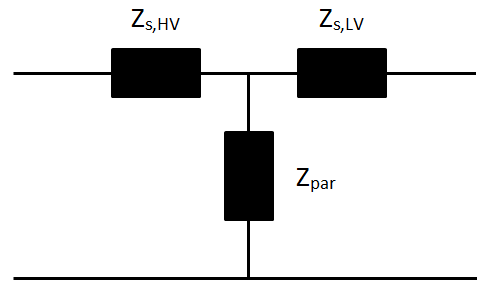
\includegraphics[width=0.65\textwidth, angle=0]{Electric/MyGraphics/trafo_equischeme.png}}
\caption{Equivalent scheme of a transformator}
\label{figTrafo}
\end{figure}

The parallel element ($Z_{par}$) is defined during a no-load test of the transformer. At the primary side, the nominal voltage is applied, while the secondary windings are open. The series elements can be neglected:
\begin{equation}
Z_{par} = \left[ \frac{400}{\sqrt{3}} \right]^2 \left[ \frac{P_0}{3} \right]^{-1}
\label{3Ploss}
\end{equation}
with $P_0$ the no-load losses.

The series elements ($Z_{s,HV}$ and $Z_{s,LV}$) are defined during short-circuit tests of the transformer. During this test, the secondary windings are shorted. Since the parallel elements are large compared to the series elements, the series elements ($Z_s = Z_{s,HV} + Z_{s,LV}$)  can be defined:
\begin{equation}
Z_s = \left[ \frac{400 u_k}{100 \sqrt{3}} \right]^2 \left[ \frac{S_n u_k}{300} \right]^{-1}
\label{3Ploss}
\end{equation}
with $S_n$ the nominal apparent power of the transformer and $u_k$ the percentage of the short-circuit voltage\footnote{The short-circuit voltage is the voltage that has to be applied at the primary winding to have the nominal current in the primary winding when the secondary winding is shorted.}. Generally, $Z_s$ is evenly distributed amongst $Z_{s,HV}$ and $Z_{s,LV}$.

The active losses in a transformer are calculated as is done in Eq.~(\ref{Ploss}) for the losses in the grid. 

\section{Electrical in-home grid}
In progress.

\section{Electrical storage}
In progress.